\documentclass[11pt, oneside]{article}   	% use "amsart" instead of "article" for AMSLaTeX format
\usepackage{geometry}                		% See geometry.pdf to learn the layout options. There are lots.
\geometry{letterpaper}                   		% ... or a4paper or a5paper or ... 
%\geometry{landscape}                		% Activate for for rotated page geometry
%\usepackage[parfill]{parskip}    		% Activate to begin paragraphs with an empty line rather than an indent
\usepackage{graphicx}				% Use pdf, png, jpg, or eps§ with pdflatex; use eps in DVI mode
								% TeX will automatically convert eps --> pdf in pdflatex		
\usepackage{amssymb}
\usepackage{amsmath}
\usepackage{parskip}
\usepackage{color}
\usepackage{hyperref}

\title{Complex Series}
%\author{The Author}
%\section{}
%\subsection*{}
\date{}							% Activate to display a given date or no date

\graphicspath{{/Users/telliott_admin/Dropbox/Tex/png/}}
% \begin{center} 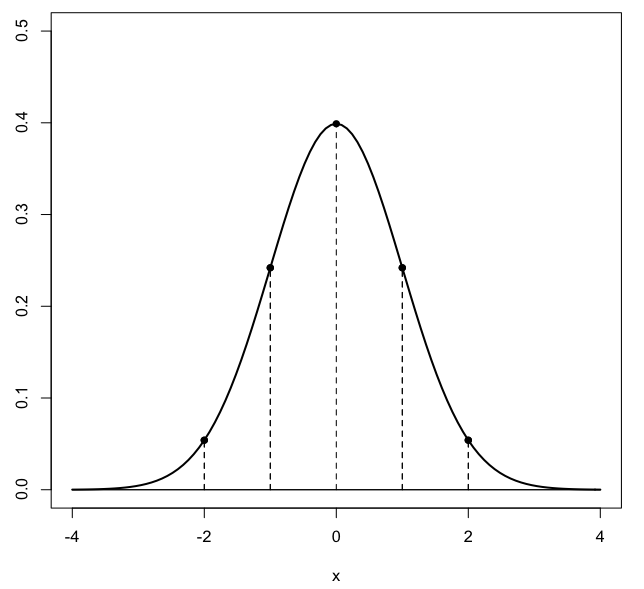
\includegraphics [scale=0.4] {gauss3.png} \end{center}
\begin{document}
\maketitle
\Large
Cauchy's theorem says that the integral around a closed path for an analytic function is zero, given some conditions.

If such a function is undefined at a limited number of points (e.g. because such values produce zero in the denominator), then those points are called poles or singularities and Cauchy 2 can be used to calculate the value of the integral (called a residue) from the value of the function at those points.

All complex functions can be expanded as power series around a fixed point $z_0$.  This is useful like if the radius of convergence is large enough to include the contour you want to integrate around.  Unlike with Taylor series, Laurent series contain terms with negative powers.  So, when integrating a function by integrating its series, we obtain a bunch of terms in different integral powers of $(z-z_0)^n$.

But by the reasoning we've given, only the term with $(z-z_0)^{-1}$ has a non-zero integral.

\subsection*{HELM}

With this writeup, we'll start working through the last section of material on complex functions produced by the HELM project.

Recall that for (most) real functions we can write them as Taylor series with terms of the form
\[ a_n (x-x_0)^n \] 
where the series is summed over positive integers from $n = 0 \rightarrow \infty$ and the coefficients are
\[ a_n = \frac{f^{(n)}}{n!} \]
the nth derivative of $f$ divided by $n!$

As an example consider
\[ f(x) = \frac{1}{1 - x} \]
This has a singularity at $x = 1$.  We can get the Taylor series expanded around $0$ for this function (this special form is called the Maclaurin series).
\[ f(x) = 1 + x + x^2 + x^3 + \dots \]
We can show that this series is equal to what we started with
\[ \frac{1}{1 - x} = 1 + x + x^2 + x^3 + \dots \]
by multiplying the right-hand side by $(1-x)$.  Imagine two long rows of numbers, one the series itself, and the second containing all the terms of the series multiplied by $-x$.  It's clear that everything cancels except the term $1$.

Alternatively, we can take derivatives and construct the series formally:
\[ f(x) = \frac{1}{1 - x} = (1-x)^{-1} \]
\[ f'(x) = \frac{1}{(1 - x)^2} = (1-x)^{-2} \]
Notice that the minus sign from the exponent cancels the minus sign from the term $(1-x)$ obtained by the chain rule.  
\[ f''(x) = \frac{2}{(1 - x)^3} \]
\[ f'''(x) = \frac{3!}{(1 - x)^4} \]
and so on.

Now, evaluated at $x_0 = 0$, these derivatives are seen to collapse to just the factorial, so we construct the terms of the series as
\[ a_n = \frac{f^{(n)}}{n!} \]
\[ = n! \ \frac{1}{n!} \]
and the factorials also cancel.  This leaves the particularly simple form:
\[ \sum_{n=0}^{\infty} x^n = 1 + x + x^2 + x^3 + \dots \]

\subsection*{Convergence}
For most series the big question is:  what is the radius of convergence?

The series expansion for real functions is centered around a fixed point $x_0$ with terms like $(x - x_0)^n$, and the series has a finite sum, only converges for $x$ sufficiently close to $x_0$.

\[ |x - x_0| < r \]

Likewise, for complex functions, series expansions will usually only be valid for a circle (or disk, or region) of convergence in the Argand plane with 
\[ | z - z_0 | < R \]
Convergence can be decided by certain tests including the ratio test and the root test (but sometimes the result is not clear).

Consider whether this complex series converges.  
\[ f(z) = \frac{1}{1 - z} \]
\[ =\sum_{n=0}^{\infty} z^n = 1 + z + z^2 + z^3 + \dots \]

Without doing any tests, we see that this is the geometric series with ratio $z$, which is known to converge when $|z| < 1$.

As the source says:  

"One of the shortcomings of Taylor series is that the circle of convergence is often only a part of the region in which $f(z)$ is analytic.  The Laurent series is an attempt to represent $f(z)$ as a series at as many points as possible. We expand the series around a point of singularity up to, but not including, the singularity itself."

Laurent series involve an annulus, usually called $D$, which is a circle that has an empty small circle in its center, like a slice through a donut.

\subsection*{Laurent's Theorem}
If $f(z)$ is analytic through a closed annulus $D$ centered at $z = z_0$, then at any point $z$ inside $D$ we can write:
\[ f(z) = a_0 + a_1(z-z_0) + a_2(z-z_0)^2 + \dots \]
\[ \hspace{27mm} + \ b_1(z-z_0)^{-1} + b_2(z-z_0)^{-2} + \dots \]
where the coefficients are given by
\[ a_n = \frac{1}{2 \pi i} \ \oint_C \frac{f(z)}{(z - z_0)^{n+1}} \ dz \]
\[ b_n = \frac{1}{2 \pi i} \ \oint_C \frac{f(z)}{(z - z_0)^{1-n}} \ dz \]

Any polynomial of $z$ is analytic, and quotients of analytic functions are also analytic.  The end result will be that the integral $\int f(z) \ dz$ may be obtained by integrating the right-hand side, where all the terms except one will have an integral equal to zero.

That is, out of this entire series given above, the only term that matters is:
\[ \oint b_1(z-z_0)^{-1} \ dz \]

\subsection*{Actually writing a Laurent Series}
Their example is the same function as before.
\[ f(z) = \frac{1}{1-z} \]

Let's sidestep the problem of determining the coefficients using the formulas given above.

Instead, just say that we seek a series expansion using negative powers of $z$, and hope to find that it will be valid in the region $|z| > 1$.

Notice that we can factor
\[ 1 - z = -z (1 - \frac{1}{z}) \]
So rewrite
\[ f(z) = \frac{1}{1-z} = -\frac{1}{z (1 - \frac{1}{z})} \]
Consider just this part
\[ \frac{1}{1 - \frac{1}{z}} \]
The trick is to see that this is equal to 
\[ 1 + \frac{1}{z} + \frac{1}{z^2} + \frac{1}{z^3} + \dots \]

One way is to say that we had before
\[ \frac{1}{1 - x} = 1 + x + x^2 + x^3 + \dots \]
Just substitute $1/z$ for $x$.  Or, perform the multiplication as we did before.  

Thus we have that
\[ f(z) = -\frac{1}{z} \ [ \ 1 + \frac{1}{z} + \frac{1}{z^2} + \frac{1}{z^3} + \dots \ ] \]
\[ \frac{1}{1-z} = - \frac{1}{z} - \frac{1}{z^2} - \frac{1}{z^3} + \dots \]

So we have a new series, which converges in a different region.

Namely, this is a geometric series with ratio $1/z$, so it converges when 
\[ \frac{1}{|z|} < 1 \]
that is, when $|z| > 1$!

Note that we can substitute $-w = z$ and get
\[ \frac{1}{1+w} =  \frac{1}{w} \ [ \ 1 - \frac{1}{w} + \frac{1}{w^2} - \frac{1}{w^3} + \dots \ ] \]
\[ \frac{1}{1+w} =  \frac{1}{w} - \frac{1}{w^2} + \frac{1}{w^3} + \dots \]
go back to $z$ as the variable
\[ \frac{1}{1+z} =  \frac{1}{z} - \frac{1}{z^2} + \frac{1}{z^3} - \frac{1}{z^4} + \dots \]
Check by multiplying the right-hand side by $z$ and see all the cancellations after the first term.

\subsection*{Poles and singularities}
The \emph{principal part} of the Laurent series is the part containing negative powers of $(z - z_0)$.  The series for different functions may have a finite number of terms or they may not.  

If the number of terms is finite like
\[ \frac{b_1}{z-z_0} + \frac{b_2}{(z-z_0)^2} + \dots + \frac{b_m}{(z-z_0)^m} \]
then we say that $f(z)$ has a pole of order $m$ at $ z = z_0$.

If there is an infinite number of terms then $z = z_0$ is called an isolated essential singularity of $f(z)$.  Also, some complex functions have non-isolated singularities called branch points. An example of such a function is $\sqrt{z}$.

A pole of order $1$ is called a simple pole, and a pole of order $2$ is called a double pole.  For example the function
\[ f(z) = \frac{i}{z(z-i)} = \frac{1}{z-i} - \frac{1}{z} \]
has a simple pole at $z = 0$ and another simple pole at $z = i$.  

\subsection*{problem}
Expand 
\[ f(z) = \frac{1}{2 - z} \]
Factor out the $1/2$ 
\[ = \frac{1}{2} \ \frac{1}{(1 - z/2)} \]
and substitute $w = z/2$.  The second term is then the same series as before
\[ \frac{1}{1-w} = - \frac{1}{w} - \frac{1}{w^2} - \frac{1}{w^3} + \dots \]
substitute back for $w = z/2$
\[ \frac{1}{1 - z/2} = - \frac{2}{z} - \frac{2^2}{z^2} - \frac{2^3}{z^3} + \dots \]
and multiply by $1/2$
\[ = - \frac{1}{z} - \frac{2}{z^2} - \frac{2^2}{z^3} + \dots \]
This is a geometric series with ratio $2/z$ so it is valid when
\[ | \frac{2}{z}|  < 1 \]
\[ |z| > 2 \]

\subsection*{The Residue Theorem}
Suppose that $f(z)$ is a function which is analytic inside and on a closed contour $C$, except for a pole of order $m$ at $z=z_0$, which lies inside $C$.

To evaluate $\oint_C f(z) \ dz$, we can expand $f(z)$ in a Laurent series in powers of $(z-z_0)$.  

If we let $\Gamma$ be a circle of center $z_0$ lying inside $C$ then
\[ \oint_C f(z) \ dz = \int_{\Gamma} f(z) \ dz \]

We know that the integral of each of the powers of $(z-z_0)$ is zero except
\[ I = \int \frac{b_1}{(z-z_0)} \ dz \]
and the value of this integral is $2 \pi i \ b_1$ by Cauchy 2.

Since it is the only coefficient remaining after integration it is called the \emph{residue} of $f(z)$ at $z = z_0$.  We rearrange the above to give
\[ b_1 = \frac{1}{2 \pi i} \ \oint_C f(z) \ dz \]

\subsection*{Finding residues}
This gets a little confusing.  Let's see if we can clarify things by working through an extremely simple example.  

As the theorem describes, suppose we find a Laurent series for $f(z)$ as
\[ f(z) = \frac{b_1}{(z-z_0)} + \sum_{n=0}^{\infty} \frac{a_n}{(z-z_0)^n} \]
with no terms in higher negative powers of $(z-z_0)$, then when we integrate
\[ \oint_{\Gamma}  f(z) \ dz = \oint \frac{b_1}{(z-z_0)} \ dz \]
because all the other powers drop out.
Furthermore, although we may not know what $b_1$ is at this point, it is a \emph{constant}.  Therefore, we can easily use Cauchy2 to integrate the right hand side.
 \[ \oint \frac{b_1}{(z-z_0)} \ dz = 2 \pi i \ b_1 \]
 we just write a constant complex function
 \[ g(z) = b_1 \]
 so 
 \[ \oint \frac{g(z)}{z-z_0)} = 2 \pi i \ g(z_0) = 2 \pi i \ b_1 \]
and
\[ b_1 = \frac{1}{2 \pi i} \ \oint_{\Gamma} \frac{f(z)}{z-z_0)} \]

\subsection*{example}
Let's say $f(z)$ has a simple pole at $z = z_0$.  For simplicity, say that 
\[ f(z) = \frac{1}{z^2 + 1} \]
The way I would solve this is to factor
\[ = \frac{A}{z - i} + \frac{B}{z + i} \]
If you do the usual manipulation, it turns out that $A = -B = 1/2i$ so
\[ \frac{1}{z^2 + 1}  = \frac{1}{2i} \ [ \frac{1}{z - i} - \frac{1}{z + i} \ ] \]
as we can easily check.

Thus, we have two single poles at $z \pm i$.  

So then if I want to integrate around a contour which includes (say) the upper pole at $z = i$, the term with $z + i$ in the denominator is not a singularity and its integral is zero.  The non-zero one is
\[ \int \frac{1}{2i} \ [ \frac{1}{z - i} \ ] \ dz \]
We use Cauchy 2 to find that the value is
\[ = 2 \pi i \ f(z_0) =  2 \pi i \ f(i) \]
\[ = 2 \pi i \ \frac{1}{2i} = \pi \]
That is
\[  \oint_C \frac{1}{z^2 + 1} \ dz = \pi \]
for $C$ enclosing $z=i$ but not $z = -i$.

Now, according to the notes I'm following, the value of the residue $b_1$ for this problem is 
\[ b_1 = \frac{1}{2i} \]
Thus
\[ I = \oint_C f(z) \ dz = 2 \pi i \ b_1 \]

The way they do this is to take the Laurent series
\[ f(z) = \frac{b_1}{(z-z_0)} + \sum_{n=0}^{\infty} a_n (z-z_0)^n \]
multiply both sides
\[ (z-z_0) \ f(z) = b_1 + \sum_{n=0}^{\infty} a_n (z-z_0)^{n+1} \]
So the $n=0$ term all subsequent terms under the sum have a factor of at least $(z - z_0)$ and they disappear when we take the limit as $z \rightarrow z_0$, leaving only:
\[ \lim_{z \rightarrow z_0} (z-z_0) \ f(z) = b_1 \]
Thus
\[ b_1 = \lim_{z \rightarrow z_0} (z-z_0) \ \frac{1}{(z - i)(z + i)} \]
In the case of the pole at $z = i$ we set $z_0 = i$ and then have
\[ = (z-i) \ \frac{1}{(z - i)(z + i)} \]
\[ = \frac{1}{z + i} = \frac{1}{2i} \]

To recap
\[  \oint_C \frac{1}{z^2 + 1} \ dz = \pi \]
for $C$ enclosing $z=i$ but not $z = -i$.
The residue $b_1$ is defined to be
\[ b_1 = \lim_{z \rightarrow z_0} (z-z_0) \ f(z)  \]
which turns out to have the value
\[ b_1 = \frac{1}{2i} \]
so we see that 
\[ \oint_C f(z) \ dz = 2 \pi i \ b_1 \]
which looks a lot like Cauchy 2.
\[ \oint_C \frac{f(z)}{z - z_0} \ dz = 2 \pi i \ f(z_0) \]
Just think of it as in the limit that $z \rightarrow z_0$, the denominator on the left is a constant, so we can multiply both sides by $z - z_0$ to obtain the result for the residue.

\subsection*{example}
\url{https://math.berkeley.edu/~nikhil/courses/121a/laurent.pdf}

Here is another example where we know the Laurent series:
\[ f(z) = z e^{1/z} \]
Use the known series expansion for the exponential to write:
\[ = z \ [ \ 1 + (1/z) + \frac{(1/z)^2}{2!} + \dots \ ] \]
\[ = z + 1 + \frac{(1/z)}{2!} + \dots \ ] \]

So the integral around 
\[ \oint f(z) \ dz = \oint \frac{(1/z)}{2!} \]
Our formulas are:
\[ b_1 = \lim_{z \rightarrow z_0} (z-z_0) \ f(z)  \]
\[ \oint f(z) \ dz = 2 \pi i \ \sum \text{ Res } \]

so the residue is
\[ b_1 = \lim_{z \rightarrow 0} (z) \ \frac{(1/z)}{2!} = \frac{1}{2} \]
and
\[ \oint f(z) \ dz = 2 \pi i \ \frac{1}{2} = \pi i \]

We don't need to actually know the Laurent series, only that it exists.  The form is
\[ f(z) = \sum_{n=0}^{\infty} a_n(z-z_0)^n + \frac{b_1}{z-z_0} + \dots + \frac{b_m}{(z-z_0)^m} \]

Now there are three steps.  Multiply by $(z - z_0)^m$
\[ (z - z_0)^m f(z) = \sum_{n=0}^{\infty} a_n(z-z_0)^{n+m} + b_1 (z-z_0)^{m-1} + \dots + b_m \]

Second, lose the $b_2, \dots b_m$ terms by differentiating $m-1$ times.  (Note the exponents for terms beyond $b_1$ are \emph{smaller}, so they disappear...
\[ \frac{d^{m-1}}{dz^{m-1}} (z-z_0)^m f(z) = \sum_{n=0}^{\infty} a_n\frac{d^{m-1}}{dz^{m-1}}  (z-z_0)^{n+m} + (m-1)! \ b_1 \]

Kill off al the $a_n$ terms by taking the limit $z \rightarrow z_0$
\[ \lim_{z \rightarrow z_0}  \frac{d^{m-1}}{dz^{m-1}} (z-z_0)^m f(z) = (m-1)! \ b_1 \]
\[ b_1 = \frac{1}{(m-1)!} \ \lim_{z \rightarrow z_0}  \frac{d^{m-1}}{dz^{m-1}} (z-z_0)^m f(z) \]

\subsection*{example}



\end{document}  